\chapter{Image Reconstruction}
- recap results of last chapter
- restate motivation of imaging
- chapter overview

\section{PyTorch}
The algorithms implemented in this chapter are presented in the PyTorch framework.
As a machine learning framework, it provides accelerated tensor processing.
Tensors, ie.\ rectangular multidimensional arrays are a perfect fit to
describe the signals sent by the sensor and the subsequent signal processing.

Since a huge part of the operations in the imaging algorithms are parallelizable,
substantial performance gains can be achieved with the built-in parallel processing
of tensor operations in PyTorch.
While parallel processing on a CPU already substantially improves runtimes,
even better performance can be achieved with GPU-enabled parallel processing,
which is currently available using the CUDA-API on NVDIA GPUs.

To aid in understanding any code listings referenced in this chapter,
refer to a brief tutorial in section \ref{sec:pytorch_tutorial}
that discusses some key parts of PyTorch's syntax for tensor processing.

\section{FFT-Based Imaging}

The first imaging algorithm to be implemented is based on the FFT.
A detailed description of the algorithm can be found in section \ref{ssec:dft_imaging_theory},
but the following is an abrigded summary to reiterate the key principles.

The range is estimated by computing the FFT spectrum of each time signal;
due to the FMCW principle, the frequency of the received signal is directly related to its range.
Then, making the assumption of planar incident waves
as well as having calibrated the array to achieve coherence between channels,
the angle of arrival can be estimated using FFTs over the ULA subset of the sensor's virtual antenna array.
The resolution can be increased by zero-padding the signal before applying the FFT.
An example implementation in PyTorch is shown in code listing \ref{lst:fft_img}.

The function \verb|calc_image| returns a 3D-image of dimension $N_{range} \times N_{azimuth} \times N_{elevation}$.
Its input consists of \verb|data|, a time data tensor of dimension $M \times K$,
the calibration weights \verb|weights| of dimension $K$, and \verb|settings|, a dictionary of settings.
\verb|settings| is expected to contain the input and output dimensions,
the indices of the ULA subset of the virtual array with gaps indicated by $-1$,
as well as the window functions to be used in each FFT.

\subsection{Offline Calibration}
To compute the angle of arrival, the input signal has to be made coherent in phase.
This is done by deviding each channel's range spectrum $Y_k(\Omega)$ by the estimate channel gain $\hat C_k e^{j\hat \varphi_k}$.
As well as aligning the phases correctly, this also equalizes the channel gains. \\

\subsection{Direction of Arrival Accuracy}
\label{ssec:fft_doa}
This section aims to illustrate the theoretical capabilities of FFT-based DoA-estimation on the iMCR.
The directivity in azimuth and elevation is simulated for multiple distances to illustrate the impact of near-field conditions.
\\

For this, the input time signal is an ideal point source (see eqn.\ \ref{eqn:ideal_scatterer}),
located at $(R,\theta=0,\phi=0)$
% , degraded with CSCG\footnote{circularly symmetric complex Gaussian} noise
% $\underline{\mathbf n} \sim \mathcal{CN}(0, \sigma^2 \mathbf I) $ and 
assuming a constant antenna gain of $\underline G_k(r,0,0)=1 \,\forall r,k$:
\begin{align}
    \underline y_k[m] =  e^{-j\dot \omega \frac{2R}{c_0} m T_s}
    % + \underline n_k[m]
    ,\,k\in[0,K-1],m\in[0,M-1]
\end{align}
\\
The image is computed for multiple distances at resolution
$N_{range} = 1024, N_{azimuth} = 2048$ and $N_{elevation} = 8$.
and evaluated at the range and evaluation bin of the scatterer.
The resulting peaks in azimuth are shown in figure \ref{fig:fft_azm_peak}.
\begin{figure}[h]
    \centering
    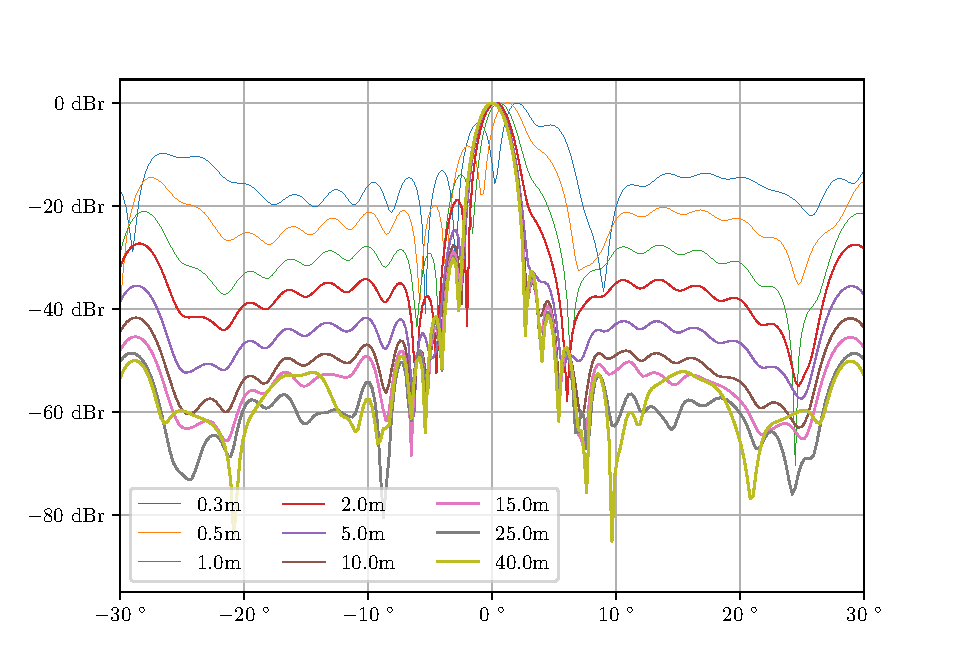
\includegraphics[width=\textwidth]{../figures/fft_azm_peak.pdf}
    \caption{iMCR FFT direction of arrival estimation: theoretical accuracy in azimuth for an ideal point scatterer at different ranges}
    \label{fig:fft_azm_peak}
\end{figure}

The Fraunhofer distance of the array can be computed from the wavelength $\lambda_0=$ \SIlist{3.944}{\mm}
and the virtual array's azimuth aperture $D_{azm} = 86 \frac{\lambda_0}{2}=$ \SI{16.96}{\cm}:
\begin{align}
    d_f  = \frac{2D_{azm}^2}{\lambda_0}
    = \SI{14.59}{\m}
\end{align}
It can be seen that for targets closer than $d_f$, the peak deteriorates in multiple ways.
The location of the peak moves to higher angles than the actual location of $\theta =$ \SI{0}{\degree}.
For targets at \SI{30}{\cm}, the peak has moved to $\theta =$ \SI{2.02}{\degree}.

In near-field conditions, the side lobe levels increase until their minimum only around \SI{20}{\dB} below the peak,
whereas in the far field, the minimum is \SI{60}{\dB} below the peak.

In far-field conditions, the main peak at $\theta =$ \SI{0}{\degree}
is clearly separated from its sidelobes by pronounced local minima.
The minimum to the right of the main peak starts to disappear below $d_f$,
and the peak to the right starts to merge with the main peak the closer the target gets.
The far-field half-power and quarter-power beamwidths are approximately
$\theta_{\SI{3}{\dB}}=$ \SI{1.9}{\degree} and $\theta_{\SI{6}{\dB}}=$ \SI{2.6}{\degree}, respectively. \\
\begin{figure}[h]
    \centering
    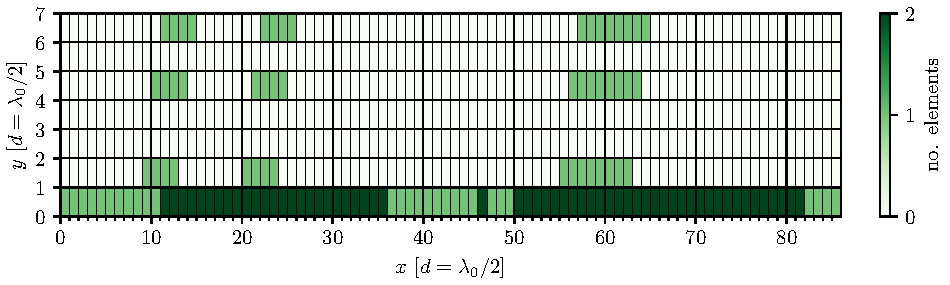
\includegraphics[width=\textwidth]{../figures/virt_array.pdf}
    \caption{iMCR virtual antenna array occupancy}
    \label{fig:virt_array}
\end{figure}

For direction of arrival estimation in azimuth, the 86-channel ULA subset of the array is well applicable to an FFT-based approach,
even with its reduced performance in near-field conditions.
Yet in elevation, such a ULA subset does not exist, as the array is sparse horizontally and vertically (c.f.\ \ref{fig:virt_array}).

To still use the FFT, an approach would be ``backfilling'' the array with zeros
to obtain a complete uniformly spaced rectangular virtual array.
The FFT is then computed over the collumns (c.f.\ \ref{fig:virt_array}) of this array,
each yielding a spectrum that is related to the direction of arrival in elevation.

A disadvantage of this approach is that it can cause substantial spectral leakage.
Our backfilled array $b[k] $ is mathematically equivalent
to applying a binary window function $w[k]$ to the ideal rectangular array $a[k]$:
\begin{align*}
    b[k]                   & =  w[k] \cdot  a[k]             \\
    \text{e.g.}\;  b[0..7] & = [b_0, b_1, 0,0,b_2,0,b_3,0 ], \\
    w[0..7]                & = [1,  1,0,0,1,0,1,0 ],         \\
    \text{and}\; a[0..7]   & = [a_0,a_1,a_2,\dots,a_7]
\end{align*}


However, this window function causes additional peaks to appear in the spectrum,
since multiplication in the time domain is equivalent to convolution in the frequency domain:
\begin{align*}
    \mathcal{F}\{b[k]\}[n] & = \mathcal{F}\{w[k] \cdot  a[k]   \}[n] \\
                           & = W[n] * A[n]
\end{align*}
In case of the example given above,
\begin{align*}
    |W[0..7]| = [4.00,\ 0.77,\ 1.41,\ 1.85,\ 2.00,\ 1.85,\ 1.41,\ 0.77]
\end{align*}

It would be possible to reduce the spectral leakage with deconvoltion algorithms.
To show the starting point for these algorithms,
the unadulterated spectral peak for targets at multiple distances is shown in figure \ref{fig:fft_elv_peak}.

\begin{figure}[h]
    \centering
    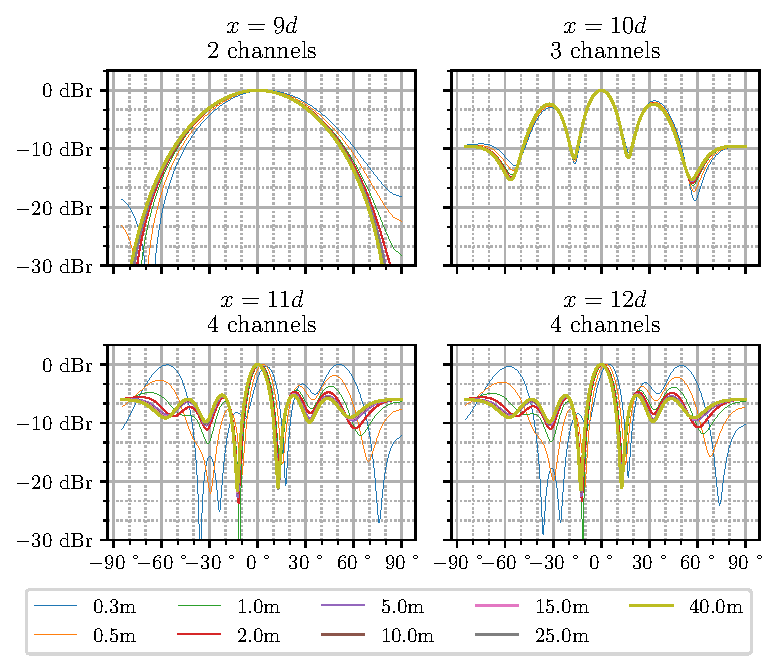
\includegraphics[width=0.8\textwidth]{../figures/fft_elv_peak.pdf}
    \caption{iMCR FFT-based direction of arrival: theoretical accuracy in elevation for an ideal point scatterer at different ranges and different array subsets}
    \label{fig:fft_elv_peak}
\end{figure}

It can be seen that the half-power beamwidth improves the more channels are included in the sub-array:
for two, three and four active channels, we approximately get
$\phi_{\SI{3}{\dB}}=$ \SIlist{60;14;12}{\degree}, respectively.

As the peak narrows, the spectrum contains more and more sidelobes.
For sub-arrays that include three channels, the side peaks are the strongest,
barely \SI{3}{\dB} less than the main peak. \\

The Fraunhofer distance of the array in elevation can be computed from the wavelength $\lambda_0=$ \SIlist{3.944}{\mm}
and the virtual array's maximal elevation aperture $D_{elv} = 7 \frac{\lambda_0}{2}=$ \SI{1.38}{\cm}:
\begin{align}
    d_f  = \frac{2D_{elv}^2}{\lambda_0}
    = \SI{9.66}{\cm}
\end{align}
The Frauenhofer distance in elevation is smaller than in azimuth by an order of magnitude.
Thus, all distances considered lie in the far-field,
and the shape of the peak should not change a lot over distance.

While this holds true for the two-- and three-channel case, if four channels are considered,
the shape does change with distance.

On the one hand, the location of the main peak moves to higher angles if the range is decreased.
On the other hand, the first two sidelobes decrease in amplitude,
while the third ones move towards $\phi=$ \SI{0}{\degree} and increase in amplitude.

TODO:

- Change Code listing

- Mention Taper Functions!!

- Conclude


\subsection{Test Image}
\label{ssec:fft_result}
To give an indication how well the theoretical capabilities of the FFT-based approach translate into real world applications,
a test scene was recorded. The sensor is placed in front of the old water tower on top of Lousberg, Aachen.
A reflector is placed slightly off-center at a distance of approximately \SI{6}{\m}.

The target 2D image spans a $24 \times$\SI{15}{\m} area in the horizontal plane,
with square pixels of edge length \SI{10}{\cm},
and the sensor located on one of the image's long sides, namely $[x,y] = [0,0]$.

It is constructed by first calculating the polar-coordinate FFT image at a resolution of $N_{range}\times N_{azimuth} = 2048 \times 512$.
% applying Hann window-functions in both fourier transforms.
The image can then be extracted from by selecting the appropriate range- and azimuth bins.
For calibration, previously measured antenna characteristics are used to improve the array's coherence.

Figure \ref{fig:fft_testimg} shows the resulting image with and without calibration.
\begin{figure}
    \centering
    \begin{subfigure}{0.8\textwidth}
        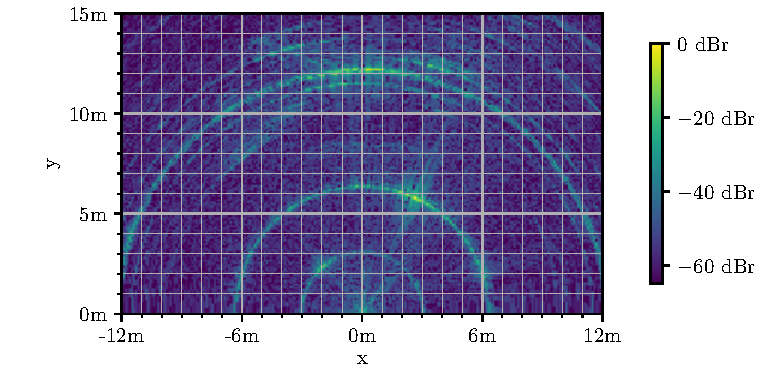
\includegraphics[width=\textwidth]{../figures/testimg_uncalibrated_fft.pdf}
        \subcaption{uncalibrated}
    \end{subfigure}
    \begin{subfigure}{0.8\textwidth}
        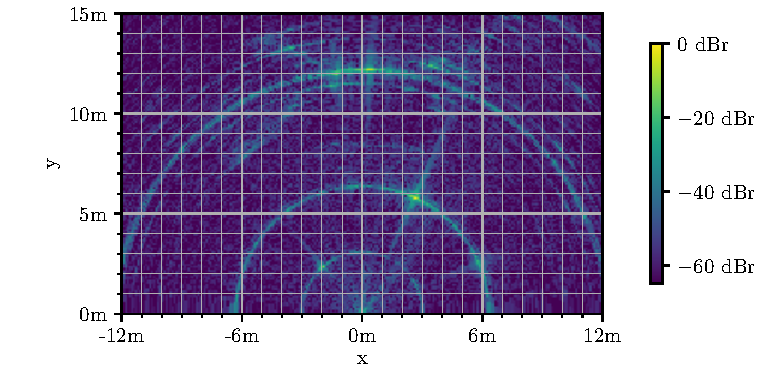
\includegraphics[width=\textwidth]{../figures/testimg_calibrated_fft.pdf}
        \subcaption{calibrated}
    \end{subfigure}
    \caption{FFT-based image generated from real data}
    \label{fig:fft_testimg}
\end{figure}
Calibration increases output SNR: less noise visible around [0m,7m]. Also reduces peak width in azimuth. Tower outline easier to make out.
Still fairly broad peaks, esp. in azimuth. CF azimuth theoretical peak: -40dB SLL. Clearer images: decrease dynamic range.

TO DO:

- image for approximate ground truth

- maybe 3d image?

- Runtime, real-time capabilities


\section{Backprojection Imaging}

The second imaging algorithm to be implemented is backprojection.
A detailed description of the algorithm can be found in section \ref{ssec:bp_imaging_theory},
but the gist of it is the following:

Backprojection works by computing the correlation between the incoming time data
and the signal of an ideal point scatterer (see eqn. \ref{eqn:ideal_scatterer})
at an arbitrary set of locations. The signal uses the measured antenna gains at that location.
Assuming the antenna gains to be static,
the ideal signals can be pre-computed to be used to generate images for multiple measurements.
An example implementation in PyTorch is shown in code listing \ref{lst:bp_img}.

TODO:

- how to calculate BP weights from measured antenna gains
\\

A major limitation of the way the backprojection algorithm is currently implemented is its scalability.
Pre-calculating the weights, while allowing for decent opportunites in decreasing the runtime through parallel processing,
quickly use a prohibitive amount of memory.

If there are $Z$ individual locations, $M$ sample points in time and $K$ channels, then $M \cdot K \cdot Z$ weights need to be computed.
For example, the weights for a uniformly spaced image with a rather low resolution of  $Z = 100 \cdot 10 \cdot 100 =$ \SI{100}{kilovoxels},
at $K=192$ and $M=1022$, stored as complex numbers consisting of two \SI{64}{bit} floating point numbers, would require
\begin{align*}
      & M \cdot K \cdot Z \cdot 2 \cdot \SI{64}{\bit} \\
    = & 1022 \cdot 192 \cdot 10^5 \cdot \SI{16}{byte} \\
    = & \SI{3.14e12}{byte} = \SI{3.14}{\tera\byte}
\end{align*}
of memory.
With the projections of Moore's law [citation needed],
this amount of memory should be available in consumer-level computers by the year 2050.
Until then, the memory requirements has to be reduced by re-computing the weights
and applying them to the input data along an arbitrary dimension.
For example, recomputing them for every of the sampled time points would reduce
the memory requirements by a factor of 1022 to only around \SI{3}{\giga\byte}.


\begin{figure}[h]
    \centering
    \begin{subfigure}[t]{\textwidth}
        \centering
        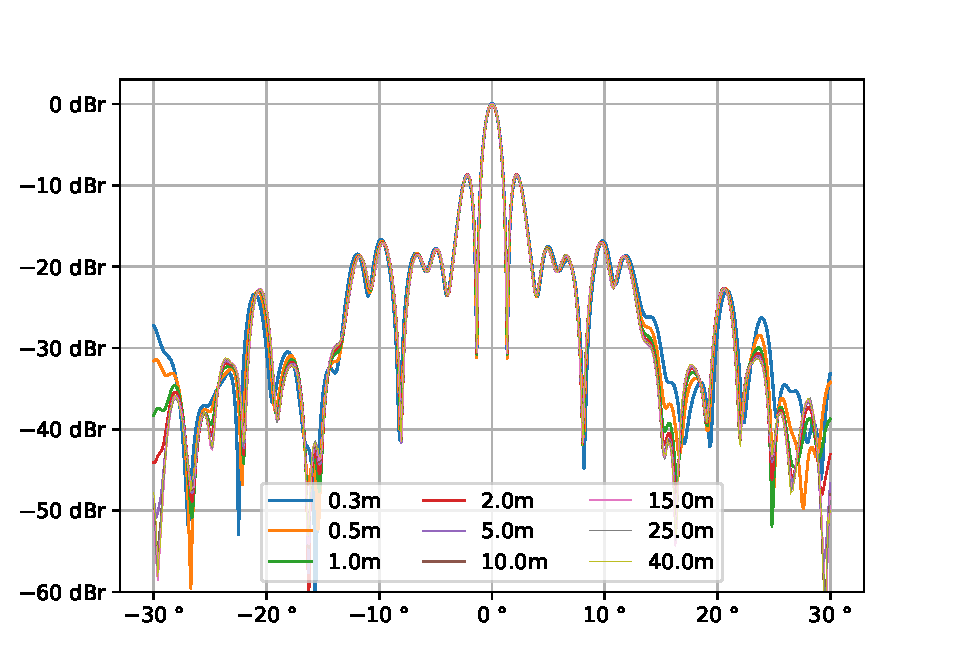
\includegraphics[width=\textwidth]{../figures/bp_azm_peak.pdf}
        \subcaption{azimuth}
        \label{fig:bp_azm_peak}
    \end{subfigure}

    \begin{subfigure}[position]{\textwidth}
        \centering
        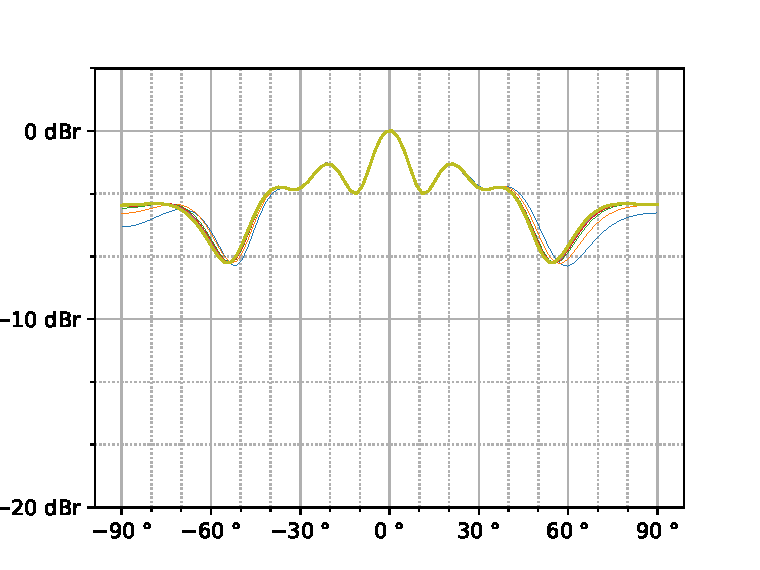
\includegraphics[width=0.8\textwidth]{../figures/bp_elv_peak.pdf}
        \subcaption{elevation}
        \label{fig:bp_elv_peak}
    \end{subfigure}

    \caption{iMCR backprojection direction of arrival estimation: theoretical accuracy for an ideal point scatterer at different ranges}
\end{figure}
\subsection{Direction of Arrival Accuracy}

To better understand the DoA-estimation capabilities of the algorithm,
the azimuth and elevation is simulated for multiple distances to illustrate the impact of near-field conditions.
The same input signal as in section \ref{ssec:fft_doa} is used.
\\

The image is computed for multiple distances at resolution
$N_{range} = 1$, ${N_{azimuth} = 512}$ and $N_{elevation} = 1$.
Naturally, the range of the image is set to the range of the ideal target each time.
The resulting peaks in azimuth and elevation are shown in figures \ref{fig:bp_azm_peak} and \ref{fig:bp_elv_peak}, respectively.


In both azimuth and elevation, it can be seen that the peak no longer deteriorates in near-field conditions.
The peak and most side lobes remain virtually identical across all considered ranges.
In azimuth, the level of the sidelobes stabilizes at around \SIrange{30}{40}{\dB} below the peak,
while in elevation, the sidelobe level is merely \SIrange{3}{6}{\dB} below the peak.

In azimuth, the half-power beamwidth is approximately $\theta_{\SI{3}{\dB}}=$ \SI{1.6}{\degree} and
the quarter-power beamwidth approximately $\theta_{\SI{6}{\dB}}=$ \SI{2.4}{\degree}.
In elevation, the half-power beamwidth is approximately $\phi_{\SI{3}{\dB}}=$ \SI{20}{\degree} and
the quarter-power beamwidth approximately $\phi_{\SI{6}{\dB}}=$ \SI{100}{\degree}.

TODO:

- discuss windowing

- discuss elevation/azimuth trade-off: should elevation-channels contribute more?


\newpage
\subsection{Test Image}
The theoretical capabilities of the backprojection algorithm are again tested for real world applications,
using the same scene as in section \ref{ssec:fft_result}.

Once again, the target 2D image spans a $24 \times$\SI{15}{\m} area in the horizontal plane,
with square pixels of edge length \SI{10}{\cm},
and the sensor located on one of the image's long sides, namely $[x,y] = [0,0]$m.
Unlike the FFT-based approach,
the backprojection algorithm allows for an arbitrary set of sample points,
so no further transformations are required.\\
\begin{figure}[t]
    \centering
    \begin{subfigure}[t]{0.8\textwidth}
        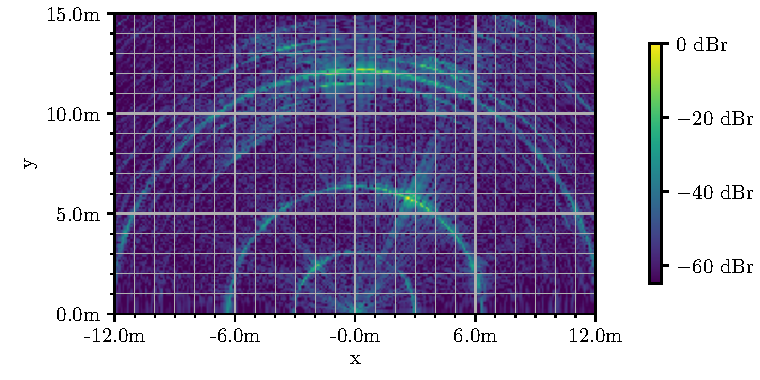
\includegraphics[width=\textwidth]{../figures/testimg_uncalibrated_bp.pdf}
        \subcaption{uncalibrated}
    \end{subfigure}
    \begin{subfigure}[t]{0.8\textwidth}
        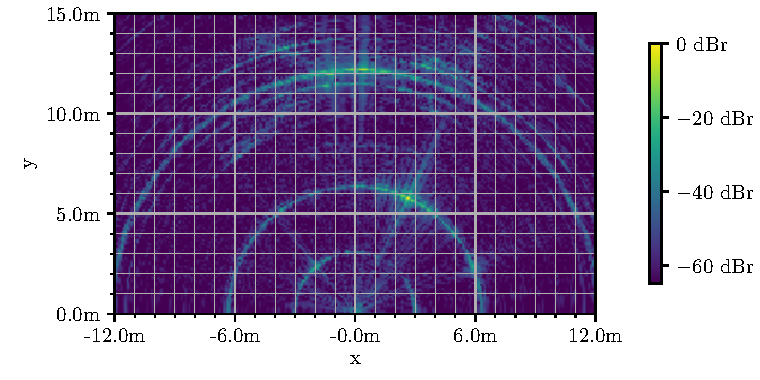
\includegraphics[width=\textwidth]{../figures/testimg_calibrated_bp.pdf}
        \subcaption{calibrated}
    \end{subfigure}
    \caption{Backprojection image generated from real data}
    \label{fig:bp_testimg}
\end{figure}
Figure \ref{fig:bp_testimg} shows the resulting image with and without calibration.
Calibration increases output SNR: less noise visible around [0m,7m].
Also reduces peak width in azimuth. Tower outline easier to make out.
Still fairly broad peaks, esp. in azimuth.
CF azimuth theoretical peak: -40dB SLL. Clearer images: decrease dynamic range.


- improve antenna gain model

- use locational calibration for test image

\section{Hybrid Approach}

Compared to the FFT-based approach, the backprojection algorithm is a lot more computationally intensive,
taking multiple orders of magnitude longer to compute a single 2D image.

    [maybe: talk about $\mathcal O(MlogN) \ll \mathcal O(MN)$]

As explained in section \ref{ssec:bp_imaging_theory},
it is possible to replace part of the computation with an FFT,
taking advantage of the increased speed and lower memory consumption of the FFT-algorithm,
while sacrificing some accuracy.

An example implementation of the backprojection-FFT-hybrid algorithm can be found in \ref{lst:hybrid_img}.
Its theoretical performance is investigated in the next section. Afterwards, a test image is computed.
\subsection{Direction of Arrival Accuracy}

- Discuss Phase error due to frequency quantization

- Plot: near-field beampattern for different FFT-lengths

\begin{figure}[h]
    \centering
    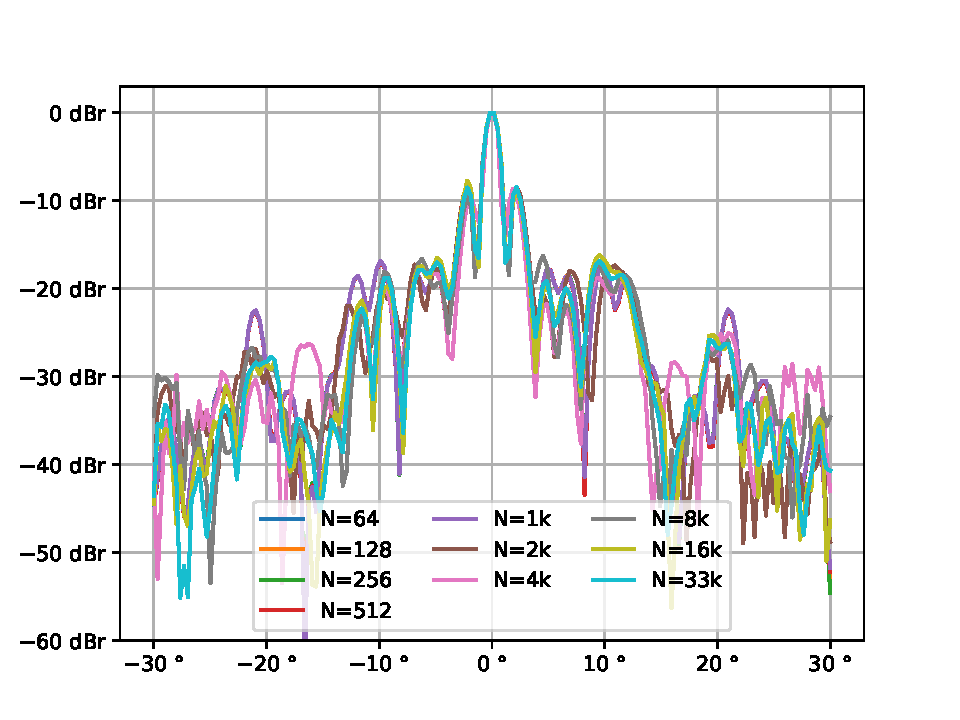
\includegraphics[width=\textwidth]{../figures/hybrid_azm_peak.pdf}
    \caption{iMCR Backprojection-FFT-Hybrid direction of arrival estimation: theoretical accuracy in azimuth for an ideal point scatterer at spectral resolutions}
    \label{fig:hybrid_azm_peak}
\end{figure}

\subsection{Test Image}

\section{Conclusion}


% 28.2.: theory
% 29.2.: stability
% 1.3.: antennas
% 2.3.: imaging
% 3.3.: Conclusion and discussion
% 4.3.: formatting, printing